\section{System Architecture}
\label{sec:architecture}

SLM~V3.3 is a modular, local-first memory system comprising 17 packages, 215 source modules, and 60 MCP tools, backed by SQLite with sqlite-vec for vector operations.

\subsection{Architecture Overview}

\begin{figure*}[t]
\centering
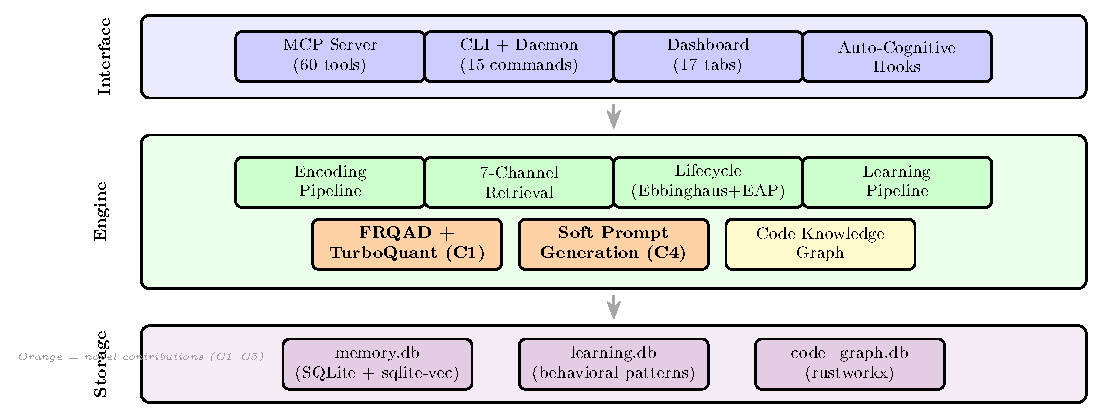
\includegraphics[width=\textwidth]{figures/fig-architecture.pdf}
\caption{SLM~V3.3 system architecture. The Interface Layer provides 60~MCP tools, a CLI with daemon serve mode (32$\times$ cold-start speedup), a 17-tab web dashboard, and auto-cognitive hooks for Claude Code. The Engine Layer implements 7-channel cognitive retrieval, Ebbinghaus lifecycle management with EAP precision scheduling, FRQAD/TurboQuant quantization (\textbf{C1}), soft prompt generation (\textbf{C4}), and a code knowledge graph module. The Storage Layer uses local SQLite databases with sqlite-vec for vector operations. Orange blocks indicate novel contributions.}
\label{fig:architecture}
\end{figure*}

The system operates in three layers:

\textbf{Interface Layer.} Four entry points:
\begin{itemize}[topsep=2pt, itemsep=1pt]
  \item \textbf{MCP Server} (60 tools including 22 code graph tools): Primary interface via the Model Context Protocol.
  \item \textbf{CLI} (15 commands): Developer-facing command line with daemon serve mode.
  \item \textbf{Dashboard}: 17-tab web UI via FastAPI for visualization and management.
  \item \textbf{Auto-Cognitive Hooks}: SessionStart, PostToolUse, and Stop hooks that automate the memory lifecycle.
\end{itemize}

\textbf{Engine Layer.} The core \texttt{MemoryEngine} orchestrates:
\begin{itemize}[topsep=2pt, itemsep=1pt]
  \item \textbf{Encoding Pipeline:} Fact extraction $\to$ entity resolution $\to$ entropy gate $\to$ emotional tagging $\to$ graph construction $\to$ consolidation (ADD/UPDATE/SUPERSEDE/NOOP).
  \item \textbf{Retrieval Pipeline:} 7-channel parallel retrieval $\to$ weighted RRF $\to$ ONNX cross-encoder reranking $\to$ Fisher-Rao re-scoring.
  \item \textbf{Lifecycle Pipeline:} Ebbinghaus decay $\to$ EAP precision scheduling $\to$ consolidation passes $\to$ soft prompt generation $\to$ garbage collection.
  \item \textbf{Learning Pipeline:} Signal collection $\to$ behavioral pattern mining $\to$ adaptive re-ranking.
\end{itemize}

\textbf{Storage Layer.} All data in local SQLite databases:
\begin{itemize}[topsep=2pt, itemsep=1pt]
  \item \texttt{memory.db}: Core fact store, knowledge graph, embeddings, temporal data, quantized embeddings, soft prompts, and forgetting schedules.
  \item \texttt{learning.db}: Behavioral patterns, feedback signals. GDPR-erasable via \texttt{slm learning reset}.
  \item \texttt{code\_graph.db}: Code knowledge graph (nodes, edges, communities, flows).
\end{itemize}

\subsection{Code Knowledge Graph}

V3.3 integrates a code knowledge graph module that bridges developer code structure with memory. The module uses tree-sitter for multi-language AST parsing, rustworkx for in-memory graph operations, and a bidirectional event bus to link code entities (functions, classes, imports) with related memories. This enables code-aware retrieval: when a developer asks about a function, SLM can retrieve not just textual memories but also the function's callers, dependencies, and related architectural decisions. The module comprises 27 source files with 385 tests, exposed through 22 dedicated MCP tools.

\subsection{Daemon Serve Mode}

V3.3 introduces a daemon serve architecture that eliminates cold-start latency. The daemon maintains a warm \texttt{MemoryEngine} instance on \texttt{127.0.0.1:8767}, auto-shutting down after 30 minutes of idle. CLI commands route through the daemon when available, falling back to direct engine instantiation otherwise.

\begin{table}[h]
\centering
\caption{Daemon serve mode performance impact.}
\small
\begin{tabular}{lrrr}
\toprule
\textbf{Operation} & \textbf{V3.2} & \textbf{V3.3 (daemon)} & \textbf{Speedup} \\
\midrule
\texttt{slm recall} (cold) & 19s & 0.6s & 32$\times$ \\
\texttt{slm recall} (warm) & 1s & 0.6s & 1.7$\times$ \\
\texttt{slm remember} (async) & 0.3s & 0.1s & 3$\times$ \\
MCP recall (cold) & 23s & $\sim$1s & 23$\times$ \\
\bottomrule
\end{tabular}
\end{table}

Data safety is ensured through a store-first pattern: \texttt{slm remember} writes to a \texttt{pending.db} SQLite store immediately ($\sim$0.1s), then processes asynchronously. Pending memories are automatically retried on engine initialization.

\subsection{Operating Modes}

\begin{itemize}[topsep=2pt, itemsep=1pt]
  \item \textbf{Mode A --- Local Guardian:} Zero-LLM operation. Embeddings via sentence-transformers subprocess. All 7 retrieval channels active. ONNX cross-encoder reranking. 70.4\% on LoCoMo.
  \item \textbf{Mode B --- Smart Local:} Adds Ollama for LLM synthesis while keeping all data local.
  \item \textbf{Mode C --- Full Power:} Cloud LLM for maximum quality. 87.7\% on LoCoMo~\cite{slm-paper2}.
\end{itemize}

% ============================================================================
% 4. COGNITIVE QUANTIZATION (C1: FRQAD + LT2E)
% ============================================================================
